\begin{marginfigure}[6cm] %MARGIN FIGURE
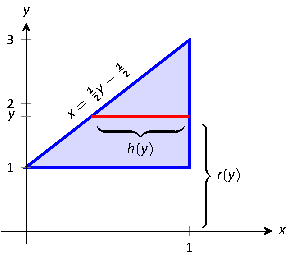
\includegraphics{figures/figshell3a}
\caption{Graphing a region in Example~\ref{eg:6.2.3}.} \label{F:6.2.Ex3a}
\end{marginfigure}

\begin{example} \label{eg:6.2.3} % EXAMPLE
Find the volume of the solid formed by rotating the region given in Example~\ref{eg:6.2.2} about the $x$-axis.

\solution
The region is sketched in Figure~\ref{F:6.2.Ex3a} with a sample differential element and the solid is sketched in Figure~\ref{F:6.2.Ex3b}. (Note that the region looks slightly different than it did in the previous example as the bounds on the graph have changed.)

The height of the differential element is an $x$-distance, between $x=\frac12y-\frac12$ and $x=1$. Thus $h(y) = 1-(\frac12y-\frac12) = -\frac12y+\frac32.$ The radius is the distance from $y$ to the $x$-axis, so $r(y) =y$. The $y$ bounds of the region are $y=1$ and $y=3$, leading to the integral

\begin{align*}
V &= 2\pi\int_1^3\left[y\left(-\frac12y+\frac32\right)\right]\ dy \\
	&= 2\pi\int_1^3\left[-\frac12y^2+\frac32y\right]\ dy \\
	&= 2\pi\left[-\frac16y^3+\frac34y^2\right]\Big|_1^3 \\
	&= 2\pi\left[\frac94-\frac7{12}\right]\\
	&=	\frac{10}{3}\pi \approx 10.472\ \text{units}^3.
\end{align*}
\end{example}

\begin{marginfigure}[-6cm] %MARGIN FIGURE
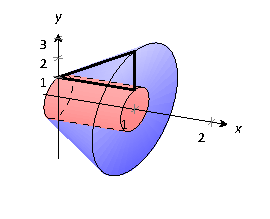
\includegraphics{figures/figshell3b}
\caption{Graphing a region in Example~\ref{eg:6.2.3}.} \label{F:6.2.Ex3b}
\end{marginfigure}